\chapter{Phylogenetic {codon} models}
{\hypersetup{linkcolor=GREYDARK}\minitoc}
\label{chap:intro-codon-models}
Evolutionary trajectories of sequences depend on the forces of mutation, selection and drift, which act conjointly such that each one of them must be well studied and understood.
More precisely, molecular evolution requires either a given selection coefficient associated to mutation, or that the fitness of each particular sequence is defined.
In other words, the relationship between sequence and fitness must be elucidated, which is the focus of the present chapter in the special case of protein-coding \acrshort{DNA} sequences.
To this aim, this chapter will first present the genetic code and classical phylogenetic codons models, which can quantify the strength of selection acting on proteins through an aggregate parameter (called $\omega$ or $\dnds$).
Application of these phylogenetic models to empirical \acrshort{DNA} alignments can be extended to model variation of selection across sites of the same protein, or between branches of a phylogenetic tree.
Subsequently, mechanistic codon models are presented, assuming that the \acrshort{DNA} sequence is at mutation-selection balance under a time-independent fitness landscape over the $20$ amino acids.
Finally, the relationship between classical and mechanistic models is investigated, and the interpretation of the discrepancy between both models is analysed.


\section{Protein coding {DNA} sequences}
\label{sec-intro:genetic-code}
Proteins have a variety of molecular and cellular roles, they are the enzymes that catalyse chemical bonds, they regulate cell processes and control their rates, they carry signals within the cell and across membranes, they bind and transport small molecules, they form cellular structures, among other functions.
This diversity of roles is accomplished by a variety of three-dimensional shapes.
A protein's three-dimensional shape is in turn determined by the linear one-dimensional sequence of amino acids of which it is made of, with protein sequences ranging from fewer than $20$ to more than $5000$ amino acids across the tree of life, with an average of about 350 amino acids.
Just as \acrshort{DNA} is oriented because of the asymmetry of nucleotides, proteins are oriented due to the asymmetry of amino acids.
One end is called the N-terminus, and the other end, the C-terminus, and each amino acid will interact with the other amino acids in its spatial vicinity.

Although each of the 20 different amino acids has unique biochemical properties, they can be classified broadly into four categories determining their solubility and acidity (classification is given in table~\ref{table:genetic_code}).
Charged amino acids can be either basic (positively charged) or acidic (negatively charged).
However, non-charged amino acids can be polar due to an uneven charge distribution, such that they can form hydrogen bonds with water.
Consequently, polar amino acids are called hydrophilic, and are often found on the outer surface of folded proteins.
Also, non-charged amino acids can have a uniform charge distribution, and do not form hydrogen bonds with water.
Reciprocally, these non-polar amino acids are called hydrophobic and tend to be found in the core of folded proteins.

\subsection{The genetic code}

Because the $20$ letter alphabet of proteins is different to the $4$ letter alphabet of nucleic acid (DNA and RNA), there is not a one-to-one correspondence between the two alphabets.
Instead, amino acids are encoded by codons, a consecutive sequence of 3 nucleotides, yielding $4^3=64$ possible permutations, more than sufficient to encode the 20 different amino acids.
Moreover, three stop codons signals the termination of the protein, such that 61 of the 64 codons are used to encode amino acids.
Since there are 61 coding codons and only 20 amino acids, there is a necessary redundancy in the code.
Thus, amino acids are encoded by synonymous codons, which are interchangeable in the sense of producing the same amino acid, with the notable exception of methionine and tryptophan, which are only encoded by a singe codon.
Altogether, the \acrshort{DNA} genetic code translating codon to amino acids, which is used almost universally by all organisms is given in table~\ref{table:genetic_code}.

\begin{table}[htbp]
    \centering
    \noindent\adjustbox{max width=\textwidth}{%
    \begin{tabular}{|c||l|c|l|c|l|c|l|c||c|}
        \hhline{|-||-|-|-|-|-|-|-|-||-|}
        & \multicolumn{2}{c|}{\textbf{T}} & \multicolumn{2}{c|}{\textbf{C}} & \multicolumn{2}{c|}{\textbf{A}} & \multicolumn{2}{c||}{\textbf{G}} & \\
        \hhline{=#========#=}
        \multirow{4}{*}{\textbf{T}} & TTT & \cellcolor{Nonpolar}                                         & TCT & \cellcolor{Polar}                                      & TAT & \cellcolor{Polar}                                          & TGT & \cellcolor{Polar}                                      & \textbf{T} \\
        \cline{2-2} \cline{4-4} \cline{6-6} \cline{8-8} \cline{10-10}
        & TTC & \cellcolor{Nonpolar} \multirow{-2}{*}{Phenylalanine (Phe/P)} & TCC & \cellcolor{Polar}                                      & TAC & \cellcolor{Polar} \multirow{-2}{*}{Tyrosine (Tyr/Y)}       & TGC & \cellcolor{Polar} \multirow{-2}{*}{Cysteine (Cys/C)}   & \textbf{C} \\
        \hhline{|~||-|-|-|>{\arrayrulecolor{Polar}}->{\arrayrulecolor{black}}|-|-|-|-||-|}
        & TTA & \cellcolor{Nonpolar}                                         & TCA & \cellcolor{Polar}                                      & TAA & \cellcolor{Stop} Stop (Ochre)                              & TGA & \cellcolor{Stop} Stop (Opal)                           & \textbf{A} \\
        \hhline{|~||-|>{\arrayrulecolor{Nonpolar}}->{\arrayrulecolor{black}}|-|>{\arrayrulecolor{Polar}}->{\arrayrulecolor{black}}|-|-|-|-||-|}
        & TTG & \cellcolor{Nonpolar}                                         & TCG & \cellcolor{Polar} \multirow{-4}{*}{Serine (Ser/S)}     & TAG & \cellcolor{Stop} Stop (Amber)                              & TGG & \cellcolor{Nonpolar} Tryptophan (Trp/W)                & \textbf{G} \\
        \hhline{|-||-|>{\arrayrulecolor{Nonpolar}}->{\arrayrulecolor{black}}|-|-|-|-|-|-||-|}
        \multirow{4}{*}{\textbf{C}} & CTT & \cellcolor{Nonpolar}                                         & CCT & \cellcolor{Nonpolar}                                   & CAT & \cellcolor{Basic}                                          & CGT & \cellcolor{Basic}                                      & \textbf{T} \\
        \cline{2-2} \cline{4-4} \cline{6-6} \cline{8-8} \cline{10-10}
        & CTC & \cellcolor{Nonpolar}                                         & CCC & \cellcolor{Nonpolar}                                   & CAC & \cellcolor{Basic} \multirow{-2}{*}{Histidine (His/H)}      & CGC & \cellcolor{Basic}                                      & \textbf{C} \\
        \hhline{|~||-|>{\arrayrulecolor{Nonpolar}}->{\arrayrulecolor{black}}|-|>{\arrayrulecolor{Nonpolar}}->{\arrayrulecolor{black}}|-|-|-|>{\arrayrulecolor{Basic}}->{\arrayrulecolor{black}}||-|}
        & CTA & \cellcolor{Nonpolar}                                         & CCA & \cellcolor{Nonpolar}                                   & CAA & \cellcolor{Polar}                                          & CGA & \cellcolor{Basic}                                      & \textbf{A} \\
        \cline{2-2} \cline{4-4} \cline{6-6} \cline{8-8} \cline{10-10}
        & CTG & \cellcolor{Nonpolar} \multirow{-6}{*}{Leucine (Leu/L)}       & CCG & \cellcolor{Nonpolar} \multirow{-4}{*}{Proline (Pro/P)} & CAG & \cellcolor{Polar} \multirow{-2}{*}{Glutamine (Gln/Q)}      & CGG & \cellcolor{Basic} \multirow{-4}{*}{Arginine (Arg/R)}   & \textbf{G} \\
        \hhline{|-||-|-|-|-|-|-|-|-||-|}
        \multirow{4}{*}{\textbf{A}} & ATT & \cellcolor{Nonpolar}                                         & ACT & \cellcolor{Polar}                                      & AAT & \cellcolor{Polar}                                          & AGT & \cellcolor{Polar}                                      & \textbf{T} \\
        \cline{2-2} \cline{4-4}\cline{6-6} \cline{8-8} \cline{10-10}
        & ATC & \cellcolor{Nonpolar}                                         & ACC & \cellcolor{Polar}                                      & AAC & \cellcolor{Polar} \multirow{-2}{*}{Asparagine (Asn/N)}     & AGC & \cellcolor{Polar} \multirow{-2}{*}{Serine (Ser/S)}     & \textbf{C} \\
        \hhline{|~||-|>{\arrayrulecolor{Nonpolar}}->{\arrayrulecolor{black}}|-|>{\arrayrulecolor{Polar}}->{\arrayrulecolor{black}}|-|-|-|-||-|}
        & ATA & \cellcolor{Nonpolar} \multirow{-3}{*}{Isoleucine (Ile/I)}    & ACA & \cellcolor{Polar}                                      & AAA & \cellcolor{Basic}                                          & AGA & \cellcolor{Basic}                                      & \textbf{A} \\
        \hhline{|~||-|-|-|>{\arrayrulecolor{Polar}}->{\arrayrulecolor{black}}|-|>{\arrayrulecolor{Basic}}->{\arrayrulecolor{black}}|-|>{\arrayrulecolor{Basic}}->{\arrayrulecolor{black}}||-|}
        & ATG & \cellcolor{Nonpolar} Methionine (Met/M)                      & ACG & \cellcolor{Polar} \multirow{-4}{*}{Threonine (Thr/T)}  & AAG & \cellcolor{Basic} \multirow{-2}{*}{Lysine (Lys/K)}         & AGG & \cellcolor{Basic} \multirow{-2}{*}{Arginine (Arg/R)}   & \textbf{G} \\
        \hhline{|-||-|-|-|-|-|-|-|-||-|}
        \multirow{4}{*}{\textbf{G}} & GTT & \cellcolor{Nonpolar}                                         & GCT & \cellcolor{Nonpolar}                                   & GAT & \cellcolor{Acidic}                                         & GGT & \cellcolor{Nonpolar}                                   & \textbf{T} \\
        \cline{2-2} \cline{4-4} \cline{6-6} \cline{8-8} \cline{10-10}
        & GTC & \cellcolor{Nonpolar}                                         & GCC & \cellcolor{Nonpolar}                                   & GAC & \cellcolor{Acidic} \multirow{-2}{*}{Aspartic acid (Asp/D)} & GGC & \cellcolor{Nonpolar}                                   & \textbf{C} \\
        \hhline{|~||-|>{\arrayrulecolor{Nonpolar}}->{\arrayrulecolor{black}}|-|>{\arrayrulecolor{Nonpolar}}->{\arrayrulecolor{black}}|-|-|-|>{\arrayrulecolor{Nonpolar}}->{\arrayrulecolor{black}}||-|}
        & GTA & \cellcolor{Nonpolar}                                         & GCA & \cellcolor{Nonpolar}                                   & GAA & \cellcolor{Acidic}                                         & GGA & \cellcolor{Nonpolar}                                   & \textbf{A} \\
        \cline{2-2} \cline{4-4} \cline{6-6} \cline{8-8} \cline{10-10}
        & GTG & \cellcolor{Nonpolar} \multirow{-4}{*}{Valine (Val/V)}        & GCG & \cellcolor{Nonpolar} \multirow{-4}{*}{Alanine (Ala/A)} & GAG & \cellcolor{Acidic} \multirow{-2}{*}{Glutamic acid (Glu/E)} & GGG & \cellcolor{Nonpolar} \multirow{-4}{*}{Glycine (Gly/G)} & \textbf{G} \\
        \hhline{|-||-|-|-|-|-|-|-|-||-|}
    \end{tabular}}
    \caption[Genetic Code]{
    The genetic code \acrshort{DNA} table translating codons into amino acids.
    Amino acids are represented into $4$ categories based on the electrochemical properties.
    Non-polar in yellow (\textcolor{Nonpolar}{\ding{110}}), polar in green (\textcolor{Polar}{\ding{110}}), basic in blue (\textcolor{Basic}{\ding{110}}) and finally acidic in red (\textcolor{Acidic}{\ding{110}}).
    Stop codons are represented in gray (\textcolor{Stop}{\ding{110}}).
    The synonymous codons encoding for the same amino acid are usually different in their third codon position, the wooble base.
    }
    \label{table:genetic_code}
\end{table}

Biochemical translation from codon to amino acid mechanistically emanates from transfer \acrshort{RNA} (\acrshort{tRNA}).
More precisely, codons binds to \acrshort{tRNA} via an anticodon, three consecutive bases that are complementary and antiparallel to the associated codon.
On the other end, a given \acrshort{tRNA} bind uniquely with one of the $20$ amino acids, where the catalytic reaction is performed by aminoacyl-tRNA synthetase~\citep{Rich1976}.
As a result, \acrshort{tRNA} genes along with aminoacyl-tRNA synthetase genes constitute the machinery necessary for translating codons into amino acids .
However, there is not a one-to-one correspondence between the $61$ codons and \acrshort{tRNA} genes.
First, the set of unique sequences of anticodon found in tRNAs genes is actually lower than $61$, and depends on the species but varies from $41$ to $55$~\citep{Goodenbour2006}.
This subset of anticodon sequences necessary to bind all $61$ codons is due to non-canonical base pairing\footnote{Canonical base pairing are A-U and G-C, where thymine (T) is replaced by uracil (U) in RNA}.
More precisely, the first two positions in the codon bond strongly to the anticodon of the \acrshort{tRNA} (second and third positions), while the third base of the codon can be subject to non-standard pairing with the first base of the anticodon.
If the anticodon contains a guanine at first position, codons with either U or C at the third position can bind to this anticodon, and this phenomenon explains why there is not any non-synonymous transition from only U to C at the third position, and why synonymous codons usually ends with T or C.
Also, if the anticodon contains an inosine at the first position, codons with either C, U or A at the third position can bind to this anticodon, such that for example leucine encoded by three codons (AUU, AUC, AUA) can be bound by the unique anticodon IAU.
Altogether, non-standard pairing explains why the number of unique anticodons is lower than the number of possible codons, and also explains some part of the structure of the genetic code.

Secondly, \acrshort{tRNA} genes with the same amino-acid binding site and anticodon, which are called isoacceptor \acrshort{tRNA}, may vary in other parts of the \acrshort{tRNA} sequence.
Effectively, many genes can code for the same isoacceptor \acrshort{tRNA}, where each gene can display varying efficiency and errors in translation, adding a layer of regulation to the process of protein synthesis~\citep{Lowe1997,Chan2008,Juhling2008,Lin2019}.
As a result, in some genes, some codons are more frequently represented than other possible synonymous codons, an effect named codon usage bias.
For genes that are expressed at high levels, the codon usage is biased in favour of the codons that have a high \acrshort{tRNA} concentration in the cell, ultimately increasing the expression rate and decreasing the rate of mistranslation by reducing the time of occupancy of an open site.
Thus, at a fine-grained molecular scope, a synonymous change can influence mRNA stability, splicing process and protein folding during translation~\citep{Plotkin2011, Rak2018}.
However in the scope of this manuscript, such selection between synonymous codons will not be considered.
Selection for proteins will be framed at the amino-acid level in a first approximation, and mutation, at the nucleotide level.

\subsection{Amino-acid transitions}

\begin{table}[htbp]
    \centering
    \noindent\adjustbox{max width=\textwidth}{%
    \begin{tabu}{|c||c|c|c|c|c|c|c|c|c|c|c|c|c|c|c|c|c|c|c|c|}
        \hline & \textbf{K} & \textbf{N} & \textbf{T} & \textbf{R} & \textbf{S} & \textbf{I} & \textbf{M} & \textbf{Q} & \textbf{H} & \textbf{P} & \textbf{L} & \textbf{E} & \textbf{D} & \textbf{A} & \textbf{G} & \textbf{V} & \textbf{Y} & \textbf{C} & \textbf{W} & \textbf{F}\\
        \hline
        \hline \textbf{K} & - & 4 & 2 & 2 & 0 & 1 & 1 & 2 & 0 & 0 & 0 & 2 & 0 & 0 & 0 & 0 & 0 & 0 & 0 & 0\\
        \hline \textbf{N} & - & - & 2 & 0 & 2 & 2 & 0 & 0 & 2 & 0 & 0 & 0 & 2 & 0 & 0 & 0 & 2 & 0 & 0 & 0\\
        \hline \textbf{T} & - & - & - & 2 & 6 & 3 & 1 & 0 & 0 & 4 & 0 & 0 & 0 & 4 & 0 & 0 & 0 & 0 & 0 & 0\\
        \hline \textbf{R} & - & - & - & - & 6 & 1 & 1 & 2 & 2 & 4 & 4 & 0 & 0 & 0 & 6 & 0 & 0 & 2 & 2 & 0\\
        \hline \textbf{S} & - & - & - & - & - & 2 & 0 & 0 & 0 & 4 & 2 & 0 & 0 & 4 & 2 & 0 & 2 & 4 & 1 & 2\\
        \hline \textbf{I} & - & - & - & - & - & - & 3 & 0 & 0 & 0 & 4 & 0 & 0 & 0 & 0 & 3 & 0 & 0 & 0 & 2\\
        \hline \textbf{M} & - & - & - & - & - & - & - & 0 & 0 & 0 & 2 & 0 & 0 & 0 & 0 & 1 & 0 & 0 & 0 & 0\\
        \hline \textbf{Q} & - & - & - & - & - & - & - & - & 4 & 2 & 2 & 2 & 0 & 0 & 0 & 0 & 0 & 0 & 0 & 0\\
        \hline \textbf{H} & - & - & - & - & - & - & - & - & - & 2 & 2 & 0 & 2 & 0 & 0 & 0 & 2 & 0 & 0 & 0\\
        \hline \textbf{P} & - & - & - & - & - & - & - & - & - & - & 4 & 0 & 0 & 4 & 0 & 0 & 0 & 0 & 0 & 0\\
        \hline \textbf{L} & - & - & - & - & - & - & - & - & - & - & - & 0 & 0 & 0 & 0 & 6 & 0 & 0 & 1 & 6\\
        \hline \textbf{E} & - & - & - & - & - & - & - & - & - & - & - & - & 4 & 2 & 2 & 2 & 0 & 0 & 0 & 0\\
        \hline \textbf{D} & - & - & - & - & - & - & - & - & - & - & - & - & - & 2 & 2 & 2 & 2 & 0 & 0 & 0\\
        \hline \textbf{A} & - & - & - & - & - & - & - & - & - & - & - & - & - & - & 4 & 4 & 0 & 0 & 0 & 0\\
        \hline \textbf{G} & - & - & - & - & - & - & - & - & - & - & - & - & - & - & - & 4 & 0 & 2 & 1 & 0\\
        \hline \textbf{V} & - & - & - & - & - & - & - & - & - & - & - & - & - & - & - & - & 0 & 0 & 0 & 2\\
        \hline \textbf{Y} & - & - & - & - & - & - & - & - & - & - & - & - & - & - & - & - & - & 2 & 0 & 2\\
        \hline \textbf{C} & - & - & - & - & - & - & - & - & - & - & - & - & - & - & - & - & - & - & 2 & 2\\
        \hline \textbf{W} & - & - & - & - & - & - & - & - & - & - & - & - & - & - & - & - & - & - & - & 0\\
        \hline \textbf{F} & - & - & - & - & - & - & - & - & - & - & - & - & - & - & - & - & - & - & - & -\\
        \hline
    \end{tabu}}
    \caption[Amino acids adjacency matrix]{
    Number of possible one nucleotide non-synonymous transitions between amino acids, integrating over the underlying codons, represented as an adjacency matrix..
    For all the possible $190$ pairs of amino acids, only $75$ pairs contains at least one non-synonymous transition.
    }
    \label{table:adjacency}
\end{table}
Because mutations are at the nucleotide level and affect only one base, any codon can have at most $9$ possible transitions to another codons as illustrated in the left panel of figure~\ref{fig:graph-codons-aa} as a graph.
Moreover, it is possible that some pairs of amino acids are not accessible through a single non-synonymous transition between the underlying codons.
In fact, most pairs of amino acids require at least two non-synonymous transitions ($114$ pairs), in comparison to pairs of amino acids that are accessible through a single non-synonymous transition ($75$ pairs).
More precisely, the number of possible transitions between the underlying codons for a pair of amino acids is determined by the adjacency matrix shown table~\ref{table:adjacency}, which is illustrated in the right panel of figure~\ref{fig:graph-codons-aa} as a graph.

\begin{figure}[htbp]
    \centering
    \begin{minipage}{0.49\linewidth}
        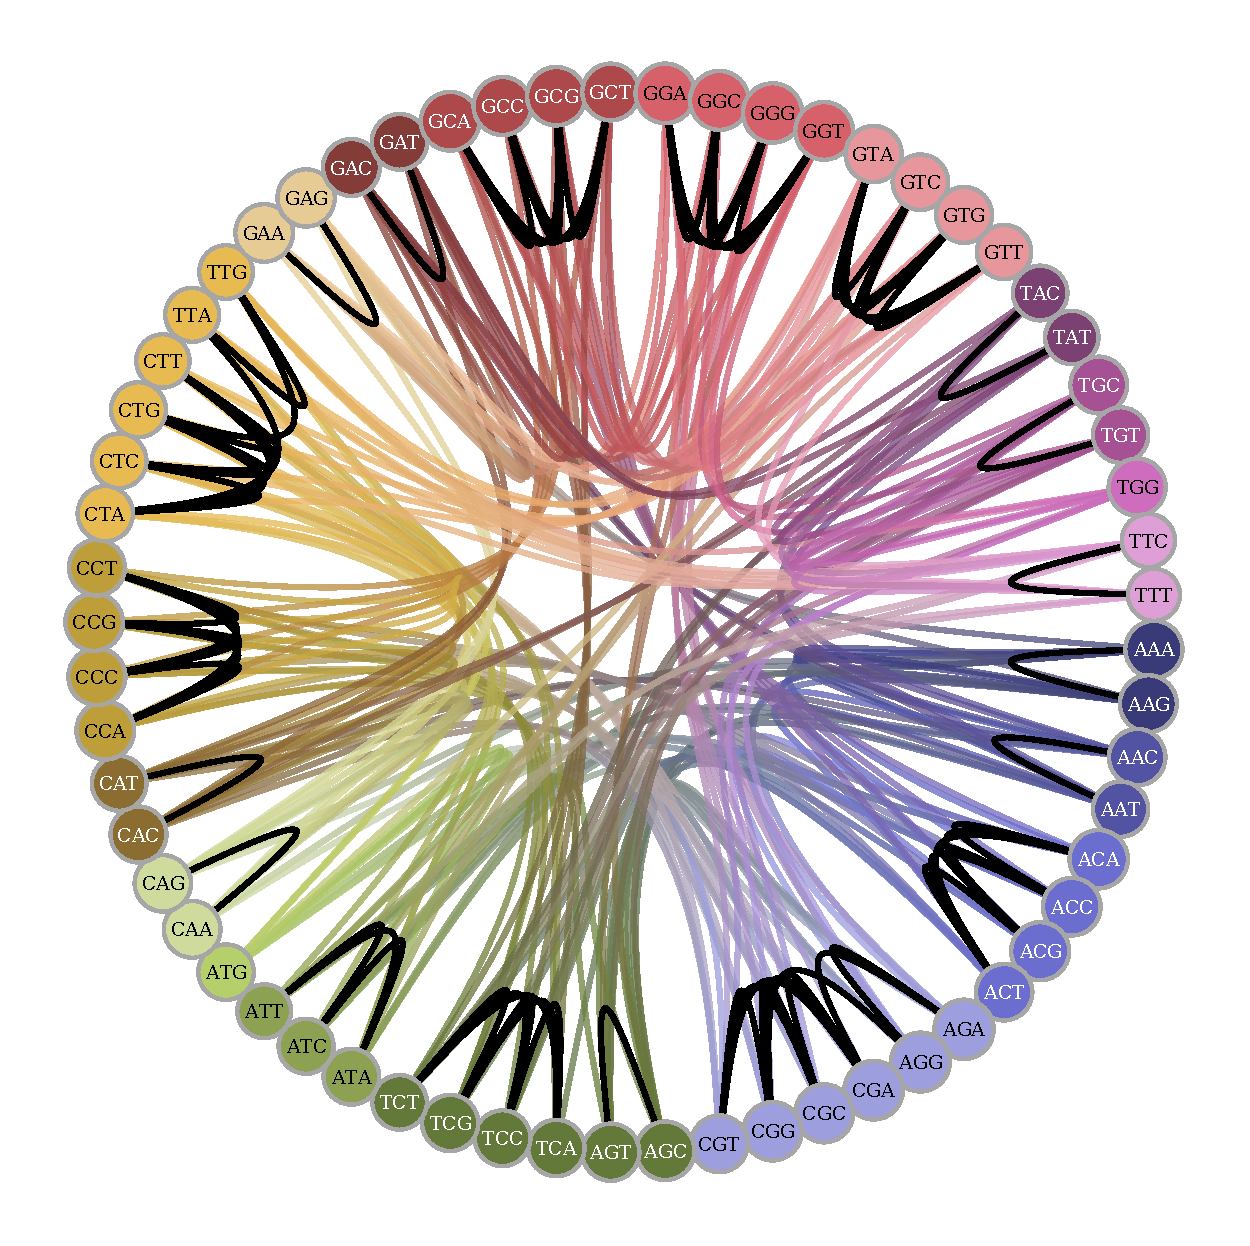
\includegraphics[width=\linewidth, page=1]{figures/gt-codon-tab20b.pdf}
    \end{minipage}%
    \hfill
    \begin{minipage}{0.49\linewidth}
        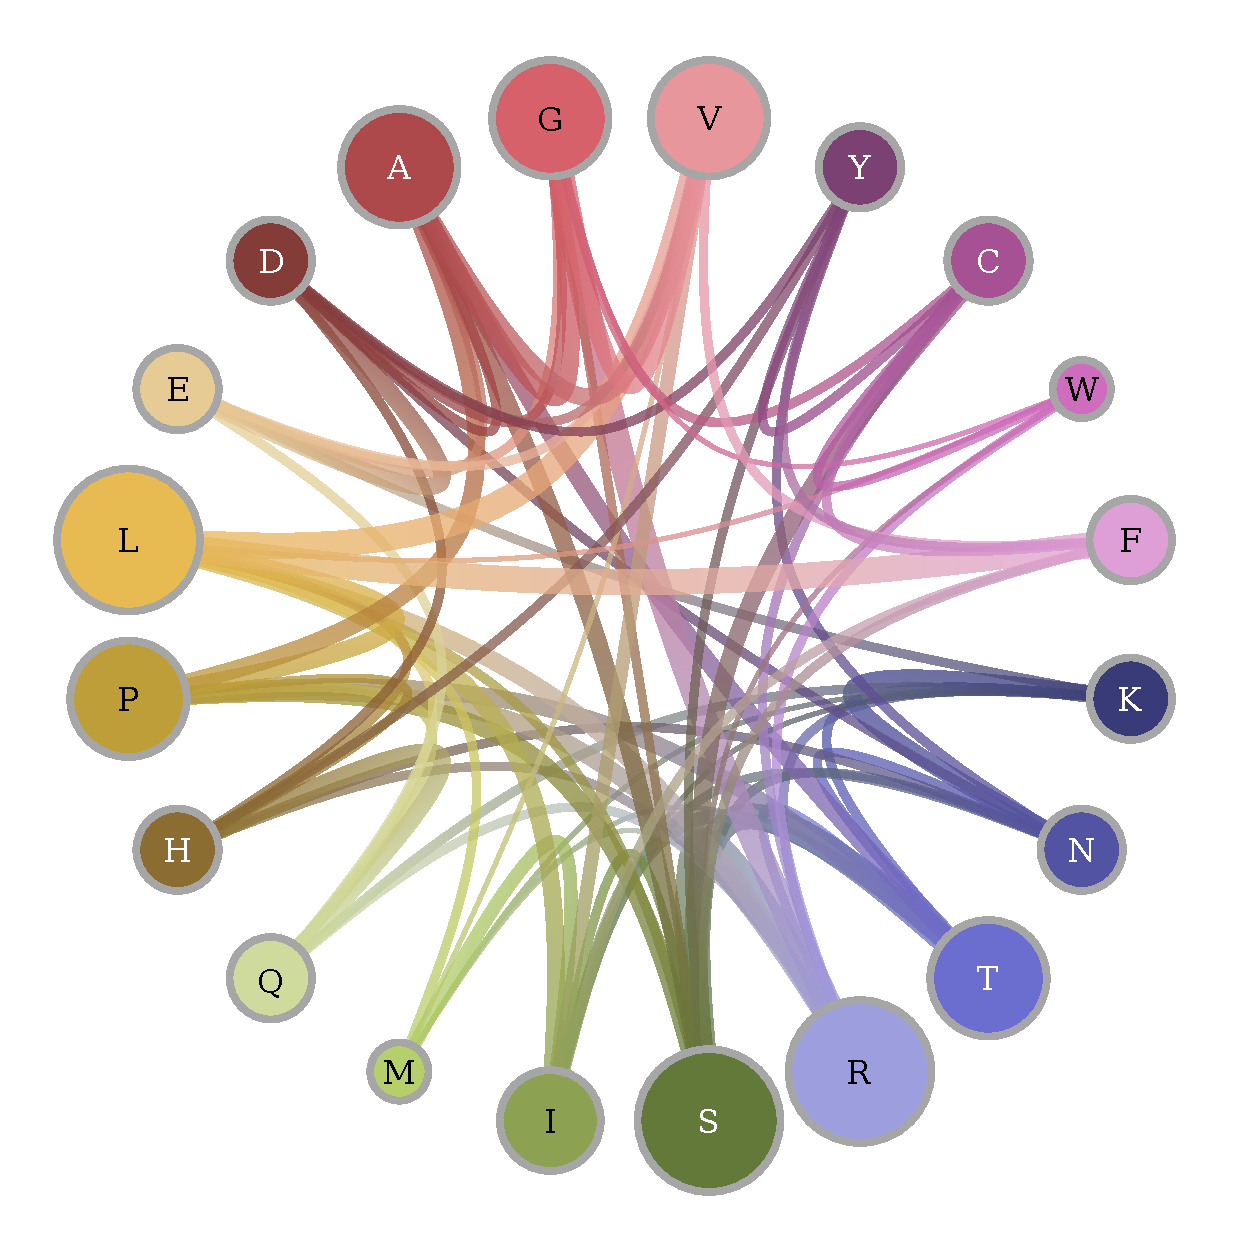
\includegraphics[width=\linewidth, page=1]{figures/gt-aa-tab20b.pdf}
    \end{minipage}

    \caption[Graphs of {codon} and amino-acid transitions]{
    Graphs of possible one nucleotide transition between codon (left panel) and between amino acids (right panel).
    Nodes correspond to codons (left panel) and amino acids (right panel), and their colour represents the encoded amino acid.
    Additionally, for amino acids, the size of nodes represents the number of underlying codons.
    An edge between two codons depicts a one nucleotide transition such that a codon can have at most $9$ possible transitions.
    Similarly, an edge between two amino acids correspond to a one nucleotide non-synonymous transition between the underlying codons, and the width of the edges represents the number of such possible transitions.
    Non-synonymous transitions are represented in a colour gradient, while synonymous transitions are depicted in black.
    The graph of the $61$ codons contains $263$ transitions, $67$ of them are synonymous while $196$ are non-synonymous.
    Codons encoding for the same amino acid are all fully connected by synonymous changes, except for serine where a transition from the set {TCT, TCG, TCC, TCA} to the set {AGT, AGC} requires passing through another amino acid, hence at least two non-synonymous transitions.
    From the perspective of amino acids, the graph of the $20$ amino acids contains $75$ non-synonymous transitions.
    The graph is not fully connected and does not form a clique. Moreover, the most distant amino acids are at most three transitions away, because a transition from methionine to tyrosine requires at least three non-synonymous transitions.
    Altogether, for all of the possible $190$ pairs of amino acids, $114$ pairs require at least two non-synonymous transitions, and one pair (M-Y) requires at least three non-synonymous transitions.
    }
    \label{fig:graph-codons-aa}
\end{figure}


\section{Classical codon models}
\label{sec:intro-classical-codon-models}

Under the approximation that selection occurs for proteins, designing substitution models at the amino-acid level has the major shortcoming of not taking into account that the underlying mutation process occurs at the nucleotide level.
Conversely, studying evolution of protein-coding \acrshort{DNA} sequences only at the nucleotide level, while disregarding the genetic code neglects the consequences that nucleotide variation can have onto protein sequences.
These shortcomings are both addressed by codon models, where the complexity of the genetic code is seen as an asset rather than an encumbrance.
Indeed the redundancy in the genetic code can be leveraged to disentangle mutation and selection in protein-coding \acrshort{DNA} sequences, under the approximation that selection occurs at the protein level in first approximation, while the mutation process occurs at the \acrshort{DNA} level.
The genetic code allows to split mutations into synonymous and non-synonymous mutations, where synonymous mutations are deemed neutral, and non-synonymous mutations are considered under selection.
Thus, by contrasting the two types of substitutions, non-synonymous against synonymous, one can estimate the impact of selection, effectively factoring out the contribution of the mutation rate and the mutation patterns.
This idea was already present in the earliest landmark contributions in molecular evolution~\citep{Kimura1968,King1969}, using simple statistical approaches.
However, the mathematical complexities created by the very irregular nature of the genetic code led to the progressive development of more sophisticated probabilistic models, formalized in a likelihood framework, in which these multiplicity issues are carefully teased apart.
The first codon models were proposed independently by \citet{Muse1994} and \citet{Goldman1994}.
The mathematical formalism is now presented in more detail.

\subsection{The Muse \& Gaut formalism}
\label{subsec:MG-formalism}

Here, we follow the formalism of codon models pioneered by \citet{Muse1994}, and further developed by \citet{Nielsen1998}.
A $4 \times 4$ mutation rate matrix $\Mutmatrix$ is first defined at the nucleotide level.
In its most general form consisting of 12 free parameters:
\begin{equation}
    \label{eq:mutrates}
    \Mutmatrix =
    \begin{blockarray}{ccccc}
        & A & C & G & T \\
        \begin{block}{c(cccc)}
            A & - & {\mutmatrix_{AC}} & {\mutmatrix_{AG}} & {\mutmatrix_{AT}} \\
            C & {\mutmatrix_{CA}} &                 - & {\mutmatrix_{CG}} & {\mutmatrix_{CT}} \\
            G & {\mutmatrix_{GA}} & {\mutmatrix_{GC}} &                 - & {\mutmatrix_{GT}} \\
            T & {\mutmatrix_{TA}} & {\mutmatrix_{TC}} & {\mutmatrix_{TG}} & - \\
        \end{block}
    \end{blockarray}
\end{equation}
By definition of the instantaneous rate matrix, the sum of the entries in each row of the nucleotide rate matrix $\Mutmatrix$ is equal to $0$, giving the diagonal entries:
\begin{equation}
    \mutmatrix_{aa} = - \sum\limits_{ b \neq a} \mutmatrix_{ab}\text{, } \forall a \in \{A,C,G,T\}
\end{equation}

Most often, this matrix is assumed to be a generalized time-reversible~\citep{Tavare1986}, or in short \acrshort{GTR}, defined by nucleotide equilibrium frequencies ($\Mutequi$) and by symmetric exchangeability rates ($\Exchan$) consisting of 9 free parameters:
\begin{equation}
    \label{eq:mutrates-GTR}
    \Mutmatrix =
    \begin{blockarray}{ccccc}
        & A & C & G & T \\
        \begin{block}{c(cccc)}
            A & - & {\exchan_{AC}\mutequi_C} & {\exchan_{AG}\mutequi_G} & {\exchan_{AT}\mutequi_T} \\
            C & {\exchan_{AC}\mutequi_A} &                        - & {\exchan_{CG}\mutequi_G} & {\exchan_{CT}\mutequi_T} \\
            G & {\exchan_{AG}\mutequi_A} & {\exchan_{CG}\mutequi_C} &                        - & {\exchan_{GT}\mutequi_T} \\
            T & {\exchan_{AT}\mutequi_A} & {\exchan_{CT}\mutequi_C} & {\exchan_{GT}\mutequi_G} & - \\
        \end{block}
    \end{blockarray}
\end{equation}

Then, grouping nucleotides into codons, the mutation rate induced by this nucleotide process from codon $\ci$ to $\cj$ depends on the underlying nucleotide change between the two codons.
Thus, if codons $\ci$ to $\cj$ are only a mutation away, let $\nucitoj$ denote the nucleotide change between them (e.g.~$\nuc(AAT, AAG) = TG$).
With this notation, the mutation rate $\mu_{\itoj}$ from codon $\ci$ to $\cj$ is:
\begin{equation}
    \mu_{\itoj} =
    \begin{dcases}
        \mutmatrix_{\nucitoj} \text{ if codons $\ci$ and $\cj$ are one mutation away,} \\
        0 \text{ else.}
    \end{dcases}
\end{equation}
In other words, the mutation rate between codons is simply the mutation rate between the underlying nucleotide change.

At the codon level, synonymous mutations are deemed neutral and the rate of synonymous substitutions ${\submatrix_{\itoj}}$ is equal to the mutation rate:
\begin{align}
    \submatrix_{\itoj} & = \mu_{\itoj}, \\
    & = \mutmatrix_{\nucitoj}.
\end{align}

In contrast, non-synonymous mutations are considered under selection such that the rate of substitution is modulated by a factor $\omega$:
\begin{align}
    \submatrix_{\itoj} & = \omega \mu_{\itoj}, \\
    & = \omega \mutmatrix_{\nucitoj}.
\end{align}

Altogether, the $61$-by-$61$ codon substitution matrix of \citet{Muse1994} is defined entirely by the mutation matrix ($\Mutmatrix$), $\omega$ and the genetic code:
\begin{equation}
    \begin{dcases}
        \submatrix_{\itoj} & = 0 \text{ if codons $\ci$ and $\cj$ are more than one mutation away,} \\
        \submatrix_{\itoj} & = \mutmatrix_{\nucitoj} \text{ if codons $\ci$ and $\cj$ are synonymous,} \\
        \submatrix_{\itoj} & = \omega \mutmatrix_{\nucitoj} \text{ if codons $\ci$ and $\cj$ are non-synonymous}.
    \end{dcases}
    \label{eq:codon-models}
\end{equation}
Again, by definition of the instantaneous rate matrix, the sum of the entries in each row of the codon substitution rate matrix $\Submatrix$ is equal to $0$, giving the diagonal entries:
\begin{equation}
    \submatrix_{\ci, \ci} = - \sum\limits_{\cj \neq \ci} \submatrix_{\itoj}.
\end{equation}

\subsection{Interpretation of the model}
\label{subsec:interpretation-of-the-model}

With the definition given above, $\omega$ identifies with the ratio of the rate of non-synonymous substitutions over the rate of synonymous substitutions, hence $\dnds$.
More globally, given how its parameterization carefully distinguishes between synonymous and non-synonymous substitutions, the model can be seen as trying to separate the effects of the mutation rates (captured by $\Mutmatrix$) and those of selection at the non-synonymous level (captured by $\omega$).

All non-synonymous mutations are considered equivalent, and $\omega$ encompasses the average strength of selection exercised on them.
Most importantly, $\omega>1$ is due to an excess in the rate of non-synonymous substitutions, indicating that the protein is under adaptive evolution.
Conversely, a default of non-synonymous substitutions, leading to $\omega<1$, means the protein is globally under purifying selection.

\subsection{Equilibrium properties}
\label{subsec:equilibrium-properties}

Under the Muse \& Gaut formalism, the codon equilibrium frequencies ($\Subequi$ depend only on the equilibrium nucleotide frequencies ($\Mutequi$), but not on $\omega$:
\begin{align}
    \subequi_{\ci} & = \dfrac{\left[\prod\limits_{k \in \{ 1, 2, 3 \}} \mutequi_{\ci[k]}\right]}{\sum\limits_{\cj}\mutequi_{\cj[1]}\mutequi_{\cj[2]}\mutequi_{\cj[3]} } \\
    & = \dfrac{\left[\prod\limits_{k \in \{ 1, 2, 3 \}} \mutequi_{\ci[k]}\right]}{(1 - \mutequi_{T}\mutequi_{A}\mutequi_{A} - \mutequi_{T}\mutequi_{A}\mutequi_{G} - \mutequi_{T}\mutequi_{G}\mutequi_{A} )}, \label{eq:equilibrium-MG}
\end{align}
where $\ci[k]$ denotes the nucleotide at position $k \in \{ 1, 2, 3 \}$ of codon $i$.

As a result of equation~\ref{eq:equilibrium-MG}, the Muse \& Gaut formalism predicts that the nucleotide composition is the same for all $3$ positions of the codons.
However it has empirically been observed that the nucleotide compositions are in fact not identical~\citep{Singer2000}.
These modulations across the three coding positions have been accommodated using the so-called 3x4 formalism~\citep{Muse1994, Goldman1994}, allowing for different nucleotide rate matrices at the three positions.
However, this is problematic, since this modelling has the consequence that synonymous substitutions occur at different rates at the first and third positions.
For instance, mutations from codon CTC to CTT or from CTA to TTA are both synonymous (leucine) and from C to T, but the 3x4 formalism would give them different rates.
Yet, in reality, the mutation process is blind to the coding structure, and should be homogeneous across coding positions, and if neutral, all mutations from C to T should have the same rate.
In any case, this suggests that the mutation matrices estimated by codon models are not correctly reflecting the mutation rates between nucleotides.

\subsection{The Goldman \& Yang formalism}
\label{subsec:GY-formalism}

In the alternative \citet{Goldman1994} formalism, the mutation rate between two codons does not depend only on the exchangeability between the underlying nucleotide change ($\exchan_{\nucitoj}$), but also on the frequency of the target codon ($\subequi_{\cj}$):
\begin{equation}
    \mu_{\itoj} = \exchan_{\nucitoj} \subequi_{\cj}.
\end{equation}

Careful examination of this model reveals a number of peculiar properties, which seem undesirable.
For example, under a mutational bias toward T, a synonymous mutation from codon AAC to AAT (asparagine) would have a lower instantaneous rate than a substitution from codon TTC to TTT (phenylalaline), both being synonymous and from C to T at third position.
In this formalism, the mutation involving a specific codon position depends on the nucleotide states at the other two positions, even if the mutation is synonymous (neutral).
Moreover, it has been shown that this alternative formalism induces different estimations of the strength of selection $\omega$~\citep{Pond2005a,Yap2010, Spielman2015}.
Altogether, such alternative formalisms are theoretically problematic, and the original Muse \& Gaut formalism remains the mechanistically justified framework~\citep{Rodrigue2008a}.

As a result, throughout this manuscript the symbol $\omega$ will be used specifically for the multiplicative factor appearing in the \citet{Muse1994} formalism (see section~\ref{subsec:MG-formalism}), whereas $\dnds$ will be used to refer generically to the ratio of non-synonymous over synonymous substitution rates, regardless of the specific formalism.
Hence, whenever $\dnds$ is used in this manuscript instead of $\omega$, the underlying specific formalism is not considered necessary to the point raised.
Contrarily, whenever $\omega$ is used, it refers to the specific Muse \& Gaut formalism of section~\ref{subsec:MG-formalism}.
A notable exception for this conventions is in the third article (chapter~\ref{chap:GenoPhenoFit} and supplementary materials in chapter~\ref{chap:GenoPhenoFit-SuppMat}), where $\omega$ will be used for readability while having a slightly different meaning (mean scaled fixation probability of non-synonymous mutations) but still identifies with the ratio of non-synonymous over synonymous substitution rates (see section~\ref{subsec:HB-formalism-nearly-neutral-model}).

\subsection{Complexification of classical codon models}
\label{subsec:classical-codon-models-complexification}

Classical models of codon substitutions have been extensively applied to protein-coding sequence alignments, to estimate the ratio of non-synonymous over synonymous substitution rates, $\dnds$.
Such models capture the average effect of selection on non-synonymous mutations, without seeking to discriminate between different types of mutations.
To circumvent such limitation, \citet{Yang1998a} introduced a codon model in which $\dnds$ depends on the distance between amino acids, measured in terms of the \citet{Grantham1974} distance.
Additionally, models introduced several $\dnds$ to account for amino-acid chemical properties (polarity, volume, charge, and so on) in classical codon models~\citep{Dutheil2008}.

One particularly important application of classical codon models has been to characterize genes under positive selection (i.e.~with a $\dnds > 1$), or sites within genes or specific lineage under accelerated evolution.
As a result, variants of codon models have been developed that can provide estimates of $\dnds$ for each site within a gene, or for each branch within a phylogenetic tree.
Moreover, these codon models have also proved to be valuable to quantify and assess the modulation of the selective constraints more generally imposed on protein-coding sequences (see section~\ref{sec:classical-codon-biophysics}).

\subsection{Variation across sites}
\label{subsec:variation-across-sites}

The strength of selection is not typically homogeneous along the protein sequence, and it has been rapidly recognized that it could be useful to estimate the $\dnds$ for each site individually, as opposed to globally over the entire sequence.
This turns out to be particularly important for detecting recurrent positive selection.
Indeed, recurrent positive selection might often be concentrated in a small region of the protein (e.g.~domain or site of the protein that is more directly interacting with a pathogen), the rest of the protein being under a regime of purifying selection.
Estimating $\dnds$ at the site level will make it possible to detect such regions under positive selection.
In contrast, the gene-level $\dnds$ will generally be below $1$.

However, the statistical information available along the tree for a specific site is sparse such that sites sharing similar patterns are merged together to gather enough signal.
Practically, in a popular approach of so-called random-site phylogenetic codon models, $\dnds$ is allowed to vary across sites, via a finite mixture model~\citep{Nielsen1998, Yang2000, Yang2005, Huelsenbeck2006}.
Generally, for detecting positive selection a category of sites is constrained to be under $\dnds > 1$.
Both proportions of sites and values of the different $\dnds$ categories are then estimated by maximum likelihood or Bayesian inference (see chapter~\ref{chap:intro-inference}).
Sites under adaptive evolution are then detected based on their empirical Bayes posterior probability $\dnds > 1$~\citep{Huelsenbeck2004,Yang2005}.
To note, in this context of site-specific finite mixture models, methods have also proposed to estimate both $\dn$ and $\ds$ separately~\citep{Pond2005a, Spielman2016}.

A long series of site models has been proposed, most of which have been implemented in \texttt{PAML}~\citep{Yang1997a,Yang2007}, but also in MrBayes for the infinite mixture version~\citep{Huelsenbeck2001, Ronquist2012}.
Specific applications at the level of the entire exome have uncovered sites of the sequence under positive recurrent selection~\citep{Kosiol2008}.
Other analyses have revealed the importance of host-pathogen or host-virus interactions in contributing to strong signals of ongoing adaptation in protein-coding sequences~\citep{Enard2016}.

Finally, independently of the question of detecting positive selection, site models also turn out to be very valuable models, in the aim of uncovering selective pressures acting on specific sites.
This can be used, for instance, to investigate the biophysical correlates of the strength of purifying selection at the site level (see section~\ref{subsec:thermo-variation-across-sites}).

\subsection{Variation across branches}
\label{subsec:variation-across-branches}

Beside variation across sites, the strength of selection is not typically homogeneous along the phylogenetic tree, and it has also been recognized that it could be useful to model this variation.
A first approach allows for a different $\dnds$ only on a given branch, or on a subset of the phylogeny, chosen a priori based on biological assumptions~\citep{Yang1998}.
For example, such models can detect an adaptive process ongoing during the divergence of one lineage, which can allow for the detection of the proteins responsible for speciation~\citep{Yang1998, Zhang2004}.
The most extreme version of this model simply assumes that each branch has its own $\dnds$, without any constraints~\citep{Popadin2007}.
To avoid overfitting, branches can be clustered based on their substitution rates, using a sequential testing approach~\citep{Dutheil2012}.

Alternatively, $\dnds$ can be modelled as a continuous trait, varying continuously along the phylogeny, and susceptible to show phylogenetic inertia.
To account for this, $\dnds$ is not mathematically formalized as a parameter anymore, but instead, it is modelled as a stochastic process, and more specifically, a log-Brownian process, splitting at each node of the tree into independent processes.
This modelling approach was previously used in the context of the comparative method, to model the evolution of quantitative traits observable at the tips~\citep{Felsenstein1985, Huelsenbeck2003}.
It was then recruited to model the variation in the total rate of substitution, in the context of the so-called auto-correlated relaxed clock models, used to estimate divergence times~\citep{Thorne1998}.
Finally, it was used to model the variation, independently, of $\ds$ and $\dn$~\citep{Seo2004}, or of $\ds$ and $\dnds$~\citep{Lartillot2011}.

The external factors determining the variation $\dnds$ across lineages have subsequently been investigated, primarily focused on environmental variables and life-history traits that can vary between species.
This has been done using either sequential approaches, first estimating the variation in $\dnds$ using some of the methods mentioned above, and then using the classical comparative method to correlate the estimated variation with independently observed quantitative or life-history traits~\citep{Popadin2007, Lanfear2010, Romiguier2014}.

Thereafter, integrative inference methods combining both molecular sequences and quantitative traits have been developed, jointly modelling the variation of all of these variables using a single multivariate Brownian process~\citep{Lartillot2011}.
Each entry of the process describes the evolution of one of the variables of interest: $\ds$, $\dnds$, quantitative traits, etc.
The model can then be fitted on an empirical data set consisting of a multiple sequence alignment of coding sequences and a matrix of quantitative traits observed in extant species.
This leads to a joint estimation of the stochastic process and the covariance matrix, thus giving estimates of the covariance between $\dnds$ and traits, corrected for phylogenetic inertia.

Applications of this integrative approach also found that $\dnds$ correlates positively with traits such as longevity and body mass~\citep{Lartillot2011, Figuet2017}.
Since lineages with a large body size and extended longevity typically correspond to low $\Ne$~\citep{Romiguier2014}, these empirical correlations suggest a negative correlation between $\dnds$ and $\Ne$, thus confirming the theoretical prediction of the nearly-neutral theory of evolution.
Similarly, and more directly, $\dnds$ was found to correlate negatively with the synonymous diversity ($\ps = 4 \Ne u$), which is a molecular proxy of effective population size~\citep{Brevet2019}.
These important results confirm one of the key predictions of the nearly-neutral theory.
However, the universality and robustness of the correlation between $\dnds$ and life-history traits is still debated, and further investigations are required~\citep{Nabholz2013,Lanfear2014,Figuet2016, Bolivar2019}.

\subsection{Variation across sites and branches}
\label{subsec:variation-across-sites-and-branches}

Naturally, both space (site-specific) and time (branch-specific) refinements mentioned above led to the development of the so-called branch-site models~\citep{Yang2002a, Zhang2004, Pond2011, Murrell2012, Murrell2013}.
The fine-grained tuning of site-branch models increased statistical power by seeking short and strong episodes of adaptive selection on a background of purifying selection.
However, in the case of Red-Queen processes ongoing on the protein, the episodes detected by branch-site models would merely be a small fraction of the underlying adaptation.
Indeed the overall tree is under adaptive process and one cannot contrast a branch to the rest of the tree.


\section{Mechanistic {codon} models}
\label{sec:intro-mechanistic-codon-models}

Classical codon models presented above capture the average effect of selection on non-synonymous mutations, without seeking to discriminate between different types of mutations.
In contrast, mechanistic codon models seek to predict individually all substitution rates, for each position and between each pair of codons, in an explicit model of the adaptive landscape.

\subsection{The Halpern \& Bruno formalism}
\label{subsec:HB-formalism}

The \citet{Halpern1998} formalism assumes that the protein-coding sequence is at mutation-selection balance under a time-independent fitness landscape, with a fitness that is multiplicative across sites (i.e.~without epistasis).
As a result, the fitness landscape is characterized by a fitness vector over the 20 amino acids at each site.
Furthermore, the substitution process at each position is independent of the current state at all other positions, and it will generally be different at each site~\citep{Rodrigue2010, Tamuri2012}.

In the following equations, I omit the dependence on sites, such that the fact that this process is site-specific is implicit.
Consider a given site, the probability of fixation depends on the difference in fitness between the amino acid encoded by the mutated codon ($\fitj$) and the amino acid encoded by the original codon ($\fiti$), where $\aai$ denotes the amino acid encoded by codon $i$.
The rate of substitution from codon $\ci$ to $\cj$ is derived from equation~\ref{eq:sub-transion-rates}:
\begin{align}
    \submatrix_{\itoj} & = \mu_{\itoj} \dfrac{4 \Ne \left({\fitj - \fiti}\right)}{{1 - \e^{4 \Ne \left({\fiti - \fitj}\right)} }}, \\
    & = \mu_{\itoj} \dfrac{\Fitj - \Fiti}{1 - \e^{\Fiti - \Fitj} }.
\end{align}

Altogether, the $61$-by-$61$ codon substitution matrix of mechanistic codon models $\Submatrix$ is defined entirely by the mutation matrix ($\Mutmatrix$), the vector of $20$ amino-acid relative fitness ($\Fit$) and the genetic code:
\begin{equation}
    \begin{dcases}
        \submatrix_{\itoj} & = 0 \text{ if codons $\ci$ and $\cj$ are more than one mutation away,} \\
        \submatrix_{\itoj} & = \mu_{\itoj} \text{ if codons $\ci$ and $\cj$ are synonymous,} \\
        \submatrix_{\itoj} & = \mu_{\itoj} \dfrac{\Fitj - \Fiti}{1 - \e^{\Fiti - \Fitj} } \text{ if codons $\ci$ and $\cj$ are non-synonymous}.
    \end{dcases}
    \label{eq:propensities-models}
\end{equation}

Because the process is time-reversible (see chapter~\ref{chap:intro-formalism}), from equation~\ref{eq:equilibrium-mut-sel}, the stationary distribution equals to:
\begin{align}
    \subequi_{\ci} & = \dfrac{\left[\prod\limits_{k \in \{ 1, 2, 3 \}} \mutequi_{\ci[k]}\right]\e^{\Fiti}}{\sum\limits_{\cj}\mutequi_{\cj[1]}\mutequi_{\cj[2]}\mutequi_{\cj[3]}\Fitj }.
\end{align}
The stationary frequency of a codon is ultimately the product of the nucleotide frequencies ($\Mutequi$) at its three positions and the scaled Wrightian fitness of the amino-acid ($\e^{\Fiti}$).

\subsection{Empirical calibration of the model}
\label{subsec:empirical-calibration-HB}

Fitting the mutation-selection model on a sequence alignment, via equation (\ref{eq:propensities-models}), results in an estimation of the nucleotide mutation rate matrix as well as the amino-acid fitness landscapes at each site of the sequence.
Several approaches have been used to do this.
In the original approach, \citet{Halpern1998} leveraged the detailed balance:
\begin{align}
    \frac{\subequi_{\ci}}{\subequi_{\cj}} & = \frac{\submatrix_{\jtoi}}{\submatrix_{\itoj}} \\
    & = \frac{\mu_{\jtoi} \left( \Fiti - \Fitj \right) \left(1 - \e^{\Fiti - \Fitj} \right)}{\mu_{\itoj}\left( \Fitj - \Fiti \right) \left(1 - \e^{\Fitj - \Fiti} \right)} \\
    & =  \frac{\mu_{\jtoi} \left(\e^{\Fiti - \Fitj} - 1 \right)}{\mu_{\itoj} \left(1 - \e^{\Fitj - \Fiti} \right)} \\
    & =  \frac{\mu_{\jtoi} \e^{\Fiti} \left(\e^{- \Fitj} - \e^{- \Fiti} \right)}{\mu_{\itoj}  \e^{\Fitj} \left(\e^{- \Fitj} - \e^{- \Fiti} \right)} \\
    & =  \e^{\Fiti - \Fitj} \frac{\mu_{\jtoi} }{\mu_{\itoj}}
\end{align}
Such that the scaled selection coefficients are related to the stationary codon frequencies:
\begin{equation}
    \Fiti - \Fitj = \ln \left( \frac{\subequi_{\ci} \mu_{\itoj} }{\subequi_{\cj} \mu_{\jtoi}} \right)
\end{equation}
And finally the substitution rate between codon $\ci$ and $\cj$ is:
\begin{align}
    \submatrix_{\itoj} & = \mu_{\itoj} \dfrac{\Fitj - \Fiti}{1 - \e^{\Fiti - \Fitj} } \\
    & = \mu_{\itoj} \frac{ \ln \left( \frac{\subequi_{\cj} \mu_{\jtoi}}{\subequi_{\ci} \mu_{\itoj} } \right) }{ 1 -  \frac{\subequi_{\ci} \mu_{\itoj} }{\subequi_{\cj} \mu_{\jtoi}} }
\end{align}
As a result, the substitution rate from codon $\ci$ to $\cj$ can be approximated based on a plugin estimator for both the mutational process and the amino-acid frequencies, independently estimated.
Alternatively, site-specific amino-acid preferences have been estimated either by penalized maximum likelihood~\citep{Tamuri2012,Tamuri2014}, or in a Bayesian context using an infinite mixture based on a Dirichlet process prior~\citep{Rodrigue2010, Rodrigue2014}.
Comparison of both inference approaches yields similar results in terms of estimated profiles and their induced selective constraint on protein-coding \acrshort{DNA} sequences~\citep{Spielman2016a}.
Finally, instead of estimating the fitness landscape directly on the multiple sequence alignment, deep mutational scanning approaches can be used to estimate fitness profiles experimentally~\citep{Bloom2014,Bloom2014a}, as presented in chapter~\ref{chap:intro-physic-proteins}.

\subsection{Modulating the fitness landscape across branches}
\label{subsec:modulating-the-fitness-landscape-across-branches}

Thus far, in the mutation-selection formalism, fitness landscape has been considered static.
In practice, fitness landscapes are dynamic and changing with time~\citep{Naumenko2012, Bazykin2015}.
In particular, selective pressures may change following one (or more) transitions to a new environment (e.g.: a new host).
Changes in selective pressures induced by environmental changes can be modelled in a mutation-selection framework by introducing different fitness profiles in different parts of the tree~\citep{Tamuri2009}.
Similarly, phenotypic convergent evolution has been investigated in relation to underlying molecular convergence at the level of codons.
In this context, if a specific codon site is responsible for the phenotypic convergence, the species sharing the convergent phenotype should also share convergence in amino-acid profiles at this specific site~\citep{Parto2018,Parto2018a}

\subsection{Mutation-selection and codon usage}
\label{subsec:model-codon-usage}

Another example of a mutation-selection mechanistic codon model is one in which codon usage bias is modelled, in particular, a model in which each synonymous codon of the same amino acids have different fitness~\citep{Yang2008}.
It is important to note that contrarily to the Halpern \& Bruno formalism, codon preferences are not site-specific but instead are estimated gene-wide.
\begin{equation}
    \begin{dcases}
        \submatrix_{\itoj} & = 0 \text{ if codons $\ci$ and $\cj$ are more than one mutation away,} \\
        \submatrix_{\itoj} & = \mutmatrix_{\nucitoj} \dfrac{\Fitcj - \Fitci}{1 - \e^{\Fitci - \Fitcj} }\text{ if codons $\ci$ and $\cj$ are synonymous,} \\
        \submatrix_{\itoj} & = \omega \mutmatrix_{\nucitoj} \dfrac{\Fitcj - \Fitci}{1 - \e^{\Fitci - \Fitcj} } \text{ if codons $\ci$ and $\cj$ are non-synonymous}.
    \end{dcases}
    \label{eq:yang-codon-models}
\end{equation}
With such a definition, this model is hybrid between the classical model (due to $\omega$) and the mechanistic mutation-selection codon model (due to the selection coefficients for codons $\Fitci$).
Such hybrid models have the interest of measuring the average effect of selection on non-synonymous mutations through $\dnds$ without making the assumption that synonymous mutations are neutral.


\section{Relationship between mechanistic and classical codon models}
\label{sec:relationship-between-mechanistic-and-classical-codon-models}

Even though classical codon models have fewer parameters than mechanistic codon models, it is important to realize they are not nested.
Indeed, it is impossible to find a given set of parameters for which the two models are equivalent, except by assuming all sites to have a uniform fitness distribution over amino acids in the Halpern \& Bruno mutation-selection model, and setting $\omega = 1$ in the Muse \& Gaut model, but this is really a trivial case.
They are inherently different and proceed from a different philosophy.
On the one hand, mechanistic models rely on an explicit fitness landscape, while, on the other hand, classical models capture the average effect of selection through a single $\omega$ parameter.

The difference can be highlighted by considering the case of reverse mutations.
In a mechanistic model (section~\ref{sec:intro-mechanistic-codon-models}), a negative selection coefficient associated with a given non-synonymous mutation is always matched by a positive selection coefficient for the reverse mutation.
As a result, the rate of substitution will be lower than the mutation rate in one direction, but higher in the other direction.
In contrast, in classical codon models (section~\ref{sec:intro-classical-codon-models}), if $\omega < 1$ (respectively, $\omega> 1$), the rate of substitution is lower (respectively, higher) than the synonymous substitution rate in the two directions.

Nevertheless, it is possible to make conceptual and quantitative connections between these two modelling paradigms.
This point was explored in detail by \citet{Spielman2015}, \citet{DosReis2015}, \citet{Jones2016} and \citet{Rodrigue2016}, summarized in table~\ref{table:params-codon-models}.

\begin{table}[htbp]
    \centering
    \noindent\adjustbox{max width=\textwidth}{%
    \begin{tabu}{|c|l|}
        \hline
        \textbf{Symbol} & \textbf{Interpretation} \\
        \hline \hline
        $\dn$ & Non-synonymous substitution rate. \\ \hline
        $\ds$ & Synonymous substitution rate. \\ \hline
        $\dnds$ & Ratio of non-synonymous over synonymous substitution rate. \\ \hline
        $\avgpfix$ & Mean scaled fixation probability of non-synonymous mutations. \\ \hline
        \multirow{2}{*}{$\omega$} & Scaling factor for all non-synonymous substitutions in the \citet{Muse1994} formalism. \\
        & Also, $\avgpfix_{\text{MG}}=\omega$ in the Muse \& Gaut formalism. \\ \hline
        $\omega_0$ & Induced $\avgpfix_{\text{HB}}$ in the \citet{Halpern1998} mechanistic formalism. \\ \hline
        $\omega_*$ & Scaling factor for all non-synonymous substitutions in the \citet{Halpern1998} formalism. \\ \hline
    \end{tabu}}
    \caption[Parameters of classical and mechanistic codon models]{Relationship between classical and mechanistic codon models}
    \label{table:params-codon-models}
\end{table}

\subsection{The Halpern \& Bruno mechanistic codon model as a nearly-neutral model}
\label{subsec:HB-formalism-nearly-neutral-model}

Once fitted to the data, the classical Muse \& Gaut (\acrshort{MG}) formalism returns estimates of mutation rates and $\omega$ (see subsection~\ref{subsec:MG-formalism}).
From there, one can compute the substitution and mutation rates of each codon substitution.
Using equation~\ref{eq:relative-sub-rate} on the subset of non-synonymous mutations thus gives $\avgpfix_{\text{MG}}$ at stationarity:
\begin{align}
    \avgpfix_{\text{MG}} & = \dfrac{ \sum\limits_{\iSetCodon} \subequi_{\ci} \sum\limits_{\cj \in \NonSyn_{\ci}} Q_{\itoj}}{\sum\limits_{\iSetCodon} \subequi_{\ci} \sum\limits_{\cj \in \NonSyn_{\ci}} \mu_{\itoj}} \\
    & = \dfrac{ \sum\limits_{\iSetCodon} \subequi_{\ci} \sum\limits_{\cj \in \NonSyn_{\ci}} \omega \mu_{\itoj}}{\sum\limits_{\iSetCodon} \subequi_{\ci} \sum\limits_{\cj \in \NonSyn_{\ci}} \mu_{\itoj}} \\
    & = \omega \dfrac{ \sum\limits_{\iSetCodon} \subequi_{\ci} \sum\limits_{\cj \in \NonSyn_{\ci}} \mu_{\itoj}}{\sum\limits_{\iSetCodon} \subequi_{\ci} \sum\limits_{\cj \in \NonSyn_{\ci}} \mu_{\itoj}} \\
    & = \omega,
\end{align}
where $\NonSyn_{\ci}$ is the set of non-synonymous codons neighbours to codon $\ci$.
Such equation is also true for any classical codon model formalism, where this identity between $\avgpfix$ and $\dnds$ bears much importance.

This rate of non-synonymous substitutions over mutations ($\avgpfix$) can be interpreted as the mean scaled fixation probability of non-synonymous mutations (see section~\ref{subsec:mean-scaled-fixation-probability}), such that even if classical codon models are not mechanistic in essence, the parameter $\dnds$ can be interpreted a posteriori as the mean scaled fixation probability of non-synonymous mutations.

On the other hand, the mechanistic codon models in the Halpern \& Bruno (\acrshort{HB}) formalism return estimates of mutation rates and fitness profiles of amino acids (see subsection~\ref{subsec:HB-formalism}).
From there, one can also compute the fixation probability individually for each codon substitution.
Likewise, using equation~\ref{eq:relative-sub-rate} on the subset of non-synonymous mutations gives ($\avgpfix_{\text{HB}}$) at stationarity:
\begin{align}
    \avgpfix_{\text{HB}} & = \dfrac{ \sum\limits_{\iSetCodon} \subequi_{\ci} \sum\limits_{\cj \in \NonSyn_{\ci}} Q_{\itoj}}{\sum\limits_{\iSetCodon} \subequi_{\ci} \sum\limits_{\cj \in \NonSyn_{\ci}} \mu_{\itoj}} \\
    & = \dfrac{ \sum\limits_{i} \subequi_{i} \sum\limits_{j \in \NonSyn_{\ci}} \dfrac{\Fitj - \Fiti}{1 - \e^{\Fiti - \Fitj} }}{\sum\limits_{i} \subequi_{i} \sum\limits_{j \in \NonSyn_{\ci} } \mu_{\itoj}}.
\end{align}
Hence, for the mutation-selection mechanistic model, $\avgpfix_{\text{HB}}$ can be interpreted as the resulting $\dnds$ induced by the model~\citep{Spielman2015,DosReis2015}.
Indeed, simulation experiments conducted by \citet{Spielman2015} under a mutation-selection model then analysed using a classical codon model indeed showed agreement between the induced and estimated $\dnds$.
To note, inference under the Muse \& Gaut formalism showed the best agreement compared to other formalisms of classical codon models.

Moreover, \citet{Spielman2015} showed mathematically that, if the underlying process is at equilibrium under a time-independent fitness landscape (nearly-neutral regime), then the mean scaled fixation probability $\avgpfix_{\text{HB}}$ induced by the model will always be lower than $1$.
In other words, they showed that mechanistic mutation-selection codon models display the important feature of genuinely accounting for purifying selection.
From a dynamic perspective, a non-synonymous mutation from a codon with high fitness to another codon will have a low probability of fixation, since the mutated codon will have a lower fitness.
At equilibrium, this low probability of fixation of the other codon results in a high frequency of the codon with higher fitness.
Essentially, at equilibrium the codon frequencies only fluctuate at the mutation-selection balance, and all the mutations are neutral on average, but slightly deleterious or advantageous, hence the name nearly-neutral models~\citep{Ohta1973, Ohta1992, Rodrigue2016}.
This justifies the interpretation of the Halpern \& Bruno mechanistic codon models as an implementation of the nearly-neutral regime.

Altogether, classical codon substitution models will interpret a mechanistic mutation-selection model as purifying selection ($\omega < 1$).
Accordingly, the mean scaled probability of fixation $\avgpfix_{\text{HB}}$ has also been denoted $\omega_0$~\citep{Rodrigue2016}.

\subsection{The Halpern \& Bruno mechanistic codon model as a nearly-neutral null model}
\label{subsec:HB-formalism-nearly-neutral-null-model}

As seen above, under the assumption that the protein is under a nearly-neutral regime, the predicted $\omega_0$ (mutation-selection model) and the estimated $\omega$ (classical model) should be the same~\citep{Spielman2015}.
But assumptions of the models can be broken, resulting in discrepancy between the $\omega_0$ induced (or predicted) by the Halpern \& Bruno mechanistic model, once fitted on the data, and $\omega$ directly estimated by classical codon models.

This deviation can be captured as a gene-wide multiplying factor $\omega_*$~\citep{Rodrigue2016}:
\begin{equation}
    \begin{dcases}
        \submatrix_{\itoj} & = 0 \text{ if codons $\ci$ and $\cj$ are more than one mutation away,} \\
        \submatrix_{\itoj} & = \mu_{\itoj} \text{ if codons $\ci$ and $\cj$ are synonymous,} \\
        \submatrix_{\itoj} & = \omega_* \mu_{\itoj} \dfrac{\Fitj - \Fiti}{1 - \e^{\Fiti - \Fitj} } \text{ if codons $\ci$ and $\cj$ are non-synonymous}.
    \end{dcases}
    \label{eq:propensities-models-omegastar}
\end{equation}
Since fitness profiles are capturing $\omega_0$, the resulting $\omega$ which is a function of the model parameters, can be interpreted as:
\begin{equation}
    \omega = \omega_* \times \omega_0
\end{equation}
This modelling approach is hybrid between mechanistic and phenomenological model, since the parameter $\omega_*$ cannot be interpreted mechanistically.
Moreover, the deviation of $\omega_*$ can bend upward or downward, where different interpretations can be given of both cases.

\subsection{Adaptive evolution}
\label{subsec:adaptive-evolution}

The Halpern \& Bruno formalism assumes that fitness landscapes are not dependent on time.
Alternatively, time-dependent fitness landscapes are known as seascape~\citep{Mustonen2009}.
Because of the movement of the fitness landscape, similarly to Red-Queen dynamics, the current sequence is more likely to slide into a fitness valley rather than on top of a peak when the landscape is moving.
In other words, because the current sequence is at mutation-selection-drift balance, they are more ways to move downward than upward in the fitness landscape.
As a result, changes of the landscape results in lower fitness of the current sequence on average.
The resulting dynamics is that selection pushes the sequence to climb up the time-dependent fitness landscape constantly, and the protein sequence is tracking a constantly moving fitness optimum.

Since the protein sequence is always lagging behind the moving target defined by the amino acid preferences, and since substitutions are accepted preferentially if they are in the direction of this target, substitutions are on average adaptive.
In other words, at the moment of a substitution the target amino acid has a high relative fitness, which can only then decrease through time.
Thus, breaking the assumption of time independence of amino-acid preferences leads to the estimation of an induced $\omega_0$ lower than the realized $\omega$:
\begin{equation}
    \omega > \omega_0 \\
    \iff \omega_* > 1
\end{equation}

\subsection{Epistasis and entrenchment}
\label{subsec:epistasis-and-entrenchment}

The nearly-neutral assumption of the Halpern \& Bruno formalism can also be broken if there is no independence between sites, known as epistasis between sites.
Unfortunately, one consequence of epistatic interactions is that even if a mutation is nearly-neutral upon fixation, subsequently fixed mutations on other sites make the original substitution more and more deleterious to revert over time~\citep{Gong2014, Lunzer2010, Mccandlish2013}.
This effect called entrenchment results in the current amino acids reinforcing their relative fitness with time, in opposition to constantly lagging behind a moving target.
In other words, at the moment of a substitution, the target amino acid has a nearly equal relative fitness, which can only increase with time~\citep{Goldstein2016, Goldstein2017}.
Contradictory to what happens during adaptation, breaking the assumption of independence between sites leads to entrenchment and the realized $\omega$ being lower than the induced $\omega_0$~\citep{Rodrigue2016}:
\begin{equation}
    \omega < \omega_0 \\
    \iff \omega_* < 1
\end{equation}

Altogether, a departure from near-neutrality with a $\omega \geq \omega_0$ is a signature of an ongoing Red-Queen process and that the protein is under ever-changing adaptation.
On the other hand, a $\omega \leq \omega_0$ is a signature of epistatic interaction between amino acids.
However, one shortcoming of nearly-neutral codon substitution models is that if one does not get a statistical departure from near-neutrality ($\omega = \omega_0$), it could be due to a mixture of both Red-Queen and epistatic processes that cannot be disentangled.